\begin{figure*}[t]
    \makebox[\textwidth][c]{
    \input{ICLR_2025/Figure_Wrappers/Legend/three_methods}
    }
    \centering
    \begin{subfigure}[b]{0.25\linewidth}
        \includegraphics[width=\textwidth]{ICLR_2025/Figures/eval_all_6_tasks/smooth_consistent_eval_Isaac-Rigid-Sliding-Multi-v0_eval_all.pdf}
    \end{subfigure}%
    \begin{subfigure}[b]{0.25\linewidth}
    \includegraphics[width=\textwidth]{ICLR_2025/Figures/eval_all_6_tasks/smooth_eval_Isaac-Rigid-Insertion-Multi-v0_eval_consistent.pdf}
    \end{subfigure}%
    %\hfill
    \begin{subfigure}[b]{0.25\linewidth}
        \includegraphics[width=\textwidth]{ICLR_2025/Figures/eval_all_6_tasks/smooth_eval_Isaac-Rigid-Insertion-Multi-Two-Actuators-v0_eval_consistent.pdf}
    \end{subfigure}%
    %\hfill
    \begin{subfigure}[b]{0.25\linewidth}
        \includegraphics[width=\textwidth]{ICLR_2025/Figures/eval_all_6_tasks/eval_30_Isaac-Rigid-Pushing-No-Contact-Multi-v0_eval_all.pdf}
    \end{subfigure}
        
    \begin{subfigure}[b]{0.25\linewidth}
        \includegraphics[width=\textwidth]{ICLR_2025/Figures/eval_all_6_tasks/smooth_eval_Isaac-Rope-Closing-v0_eval_all.pdf}
    \end{subfigure}
    %\hfill
    \begin{subfigure}[b]{0.25\linewidth}
        \includegraphics[width=\textwidth]{ICLR_2025/Figures/eval_all_6_tasks/smooth_eval_Isaac-Rope-Shaping-v0_eval_all.pdf}
    \end{subfigure}
    %\hfill
    \begin{subfigure}[b]{0.25\linewidth}
        \includegraphics[width=\textwidth]{ICLR_2025/Figures/eval_all_6_tasks/smooth_eval_Isaac-Cloth-Hanging-Multi-v0_eval_all.pdf}
    \end{subfigure}
    
    \caption{\update{Evaluation} curves for our \rebuttal{seven} manipulation tasks, comparing HEPi (ours), EMPN, and Transformer baselines. Results are averaged over 10 seeds, using IQM with 95\% confidence intervals. HEPi consistently outperforms EMPN and Transformer in tasks requiring complex exploration and heterogeneity handling, such as \textit{rigid-insertion-two-agents-3D}, \rebuttal{\textit{rigid-pushing-2D}} and \textit{cloth-hanging-3D}.}
    \vspace{-0.2cm}
    \label{fig:results_main_6_tasks}
\end{figure*}

In the main evaluations, we generate 1000 scenes per task (sampled according to Appendix~\ref{appx:task_details}) and compute the undiscounted return over 10 seeds, and report the average using Interquartile Mean (IQM) \citep{agarwal2021iqm} with 95\% confident interval. Figure \ref{fig:results_main_6_tasks} shows the \update{evaluation} curves for the \rebuttal{seven} manipulation tasks. Overall, both EMPN and HEPi outperform the Transformer in terms of sample complexity, owing to their ability to exploit symmetry.

For final performance on rigid tasks, firstly in \textit{rigid-slding-2D} and \textit{rigid-insertion-2D+z} tasks, HEPi and Transformer policies perform comparably, suggesting that the limited task complexity does not fully leverage the benefits of equivariant constraints. However, when the search space grows larger, as in the case of \textit{rigid-insertion-two-agents-3D}, Transformer struggles to find a policy that generalizes to all poses. EMPN, on the other hand, gets stuck in local optima due to its lack of expressiveness, especially in tasks requiring more exploration, such as \rebuttal{\textit{rigid-pushing-2D}}, \textit{rigid-insertion-2D+z} and \textit{rigid-insertion-two-agents-3D}. In contrast, HEPi’s explicit handling of heterogeneity allows for more effective exploration, leading to better overall performance.

In \textit{rope-closing} and \textit{rope-shaping}, simple deformable object tasks, the Transformer exhibits poor generalization, likely due to the complexity introduced by non-rigid constraints and random orientations. HEPi and EMPN perform similarly on the 2D tasks, but as tasks scale up to 3D environments, such as \textit{cloth-hanging-3D}, HEPi shows a significant advantage, outperforming both baselines. This highlights the importance of explicitly capturing heterogeneity and task geometry in manipulation. % tasks.

\begin{figure*}[t]
    \makebox[\textwidth][c]{
    \input{ICLR_2025/Figure_Wrappers/Legend/equi_five_methods}
    }
    \centering
    \begin{subfigure}[b]{0.32\linewidth}
        \includegraphics[width=\textwidth]{ICLR_2025/Figures/eval_cloth_hanging_equi/eval_full_Isaac-Cloth-Hanging-Multi-v0_eval_all.pdf}
        \caption{Original 3D Space} 
    \end{subfigure}
    \hfill
    \begin{subfigure}[b]{0.32\linewidth}
        \includegraphics[width=\textwidth]{ICLR_2025/Figures/eval_cloth_hanging_equi/eval_half_yaw_Isaac-Cloth-Hanging-Multi-v0_eval_all.pdf}
        \caption{2D Half Circle}
    \end{subfigure}
    \hfill
    \begin{subfigure}[b]{0.32\linewidth}
        \includegraphics[width=\textwidth]{ICLR_2025/Figures/eval_cloth_hanging_equi/eval_quater_yaw_Isaac-Cloth-Hanging-Multi-v0_eval_all.pdf}
        \caption{2D Quarter Circle}
    \end{subfigure}
    \caption{
    \update{
    Performance of different models on the \emph{Cloth-Hanging} task across varying sample spaces. Overall, performance improves as the sample space decreases. In terms of final performance, heterogeneous models outperform homogeneous baselines in most cases, demonstrating the benefits of explicit heterogeneity modeling. Additionally, applying equivariant constraints is critical for achieving superior performance in 3D tasks. More results can be found in Appendix~\ref{appx:further_exp}.
    }
    }
    \vspace{-0.2cm}
    \label{fig:eval_equi}
\end{figure*}



\paragraph{Generalizability}

\begin{figure*}[t]
    \begin{minipage}{0.55\textwidth}
        \centering
        \begin{subfigure}[b]{\linewidth}
            \includegraphics[width=\textwidth]{ICLR_2025/Figure_Wrappers/appx_rigid_pushing/eval_noise_inversey_heatmap_Isaac-Rigid-Pushing-No-Contact-Multi-v0_eval_all.pdf}
        \end{subfigure}
    \end{minipage}
    % \hspace{-1.0cm}
    \begin{minipage}{0.44\textwidth}
        \begin{center}
        \makebox[0.5\textwidth][c]{
            \input{ICLR_2025/Figure_Wrappers/Legend/two_methods}
        }
        \begin{subfigure}[b]{0.49\linewidth}
            \includegraphics[width=\textwidth]{ICLR_2025/Figures/eval_generalization_rigid/eval_line_Isaac-Rigid-Sliding-Multi-v0_eval_unseen_onl3_wTAE_norect.pdf}
        \end{subfigure}
        \hfill
        \begin{subfigure}[b]{0.49\linewidth}
            \includegraphics[width=\textwidth]{ICLR_2025/Figures/eval_generalization_rigid/eval_line_Isaac-Rigid-Insertion-Multi-v0_eval_unseen_onl3_wT_norect.pdf}
        \end{subfigure}
        \end{center}
    \end{minipage}
    
    \caption{\rebuttal{\textbf{Left:} Analysis of noise sensitivity and scalability to high-resolution objects in the \emph{Rigid-Pushing} task. Heatmaps show average returns under varying levels of artificial Gaussian noise in position and velocity inputs for both low-resolution and high-resolution objects. A single HEPi agent, trained on a low-resolution with additive Gaussian Noise ($\sigma = 0.01$), was used for all evaluations.     
    \textbf{Right:} Generalization performance on \emph{Rigid-Sliding} and \emph{Rigid-Insertion} tasks. Models are trained on one object (\textit{plus}), two objects (\textit{plus}, \textit{star}), and three objects (\textit{plus}, \textit{star}, \textit{pentagon}) and tested on the remaining unseen objects. Overall, \model generalizes well to unseen objects, performs consistently across resolutions, and handles noise effectively, making it suitable for real-world tasks.}
    }
    \vspace{-0.2cm}
    \label{fig:genealizability_main}
\end{figure*}


Figure~\ref{fig:eval_equi} compares the performance of different models on the \emph{Cloth-Hanging} task across varying sample spaces. As expected, smaller sample spaces simplify the exploration and improve performance. Heterogeneous models (HeteroGNN and HEPi) consistently achieve higher final returns than their homogeneous counterparts, demonstrating greater expressiveness. However, HeteroGNN requires more samples, whereas HEPi's use of \gls{empn} significantly improves sample efficiency by leveraging equivariant constraints in large 3D spaces.

Next, we evaluate the robustness of HEPi to noisy inputs and its ability to handle high-resolution object meshes on the \emph{Rigid-Pushing} task. GNNs naturally capture locality through message passing, allowing them to scale effectively to higher-resolution graphs without retraining \citep{li2020multipole, freymuth2023swarm}. During training, we added Gaussian noise ($\sigma=0.01$) to normalized positions and velocities to encourage diverse node representations, a common GNN regularization technique \citep{godwin2022simple}. The best HEPi agent was then evaluated with varying Gaussian noise levels applied to pre-normalized inputs (environment noise) and across low-resolution (\(\sim20\) nodes) and high-resolution (\(\sim1200\) nodes) object meshes. As shown in Figure~\ref{fig:genealizability_main} (left), HEPi maintains high performance across resolutions with only mild degradation at higher noise levels, demonstrating its scalability and robustness to noisy and diverse object representations.

Finally, we evaluate the generalization of these models to unseen objects on two rigid tasks: \emph{rigid-sliding} and \emph{rigid-insertion}. Both tasks are trained on subsets of objects—one (\textit{plus}), two (\textit{plus}, \textit{star}), and three (\textit{plus}, \textit{star}, \textit{pentagon})—and tested on the remaining objects. Figure~\ref{fig:genealizability_main} (right) shows that HEPi generalizes better than the Transformer baseline, benefiting from the ability of graph-based models to exploit object topology. In contrast, Transformers lack structure-aware embeddings and struggle with graph-structured inputs, as noted in prior work \citep{hong2022structureaware}.

\paragraph{Attention}

\begin{figure*}[t]
    \centering
       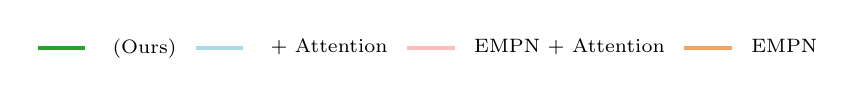
\begin{tikzpicture}
    \tikzstyle{every node}=[font=\scriptsize]
    \definecolor{tabblue}{RGB}{31, 119, 180}
\definecolor{taborange}{RGB}{255, 127, 14}
\definecolor{tabgreen}{RGB}{44, 160, 44}
\definecolor{tabred}{RGB}{214, 39, 40}
\definecolor{tabpurple}{RGB}{148, 103, 189}
\definecolor{tabbrown}{RGB}{140, 86, 75}
\definecolor{tabpink}{RGB}{227, 119, 194}
\definecolor{tabgray}{RGB}{127, 127, 127}
\definecolor{tabolive}{RGB}{188, 189, 34}
\definecolor{tabcyan}{RGB}{23, 190, 207}
\definecolor{lightblue}{RGB}{173, 216, 230}
\definecolor{sandybrown}{RGB}{244, 164, 96}
\definecolor{darkgrey}{RGB}{169, 169, 169}
\definecolor{dimgrey}{RGB}{105, 105, 105}
\definecolor{olivedrab}{RGB}{107, 142, 35}
\definecolor{darkviolet}{RGB}{148, 0, 211}
\definecolor{darkgoldenrod}{RGB}{184, 134, 11}
\definecolor{darkblue}{RGB}{0, 0, 139}
\definecolor{orchid}{RGB}{218, 112, 214}

    \begin{axis}[%
        hide axis,
        xmin=10,
        xmax=50,
        ymin=0,
        ymax=0.1,
        legend style={
            draw=white!15!black,
            legend cell align=left,
            legend columns=4,
            legend style={
                draw=none,
                column sep=1ex,
                line width=1pt,
            }
        },
        ]
        \addlegendimage{line legend, tabgreen, ultra thick} % Thicker line here
        \addlegendentry{\textbf{\model} (Ours)}
        \addlegendimage{line legend, lightblue, ultra thick} % Thicker line here
        \addlegendentry{\textbf{\model} + Attention}
        \addlegendimage{line legend, pink, ultra thick} % Thicker line here
        \addlegendentry{EMPN + Attention}
        \addlegendimage{line legend, sandybrown, ultra thick} % Thicker line here
        \addlegendentry{EMPN}
    \end{axis}
\end{tikzpicture}

        \centering
        \begin{subfigure}[b]{0.24\linewidth}
            \includegraphics[width=\textwidth]{ICLR_2025/Figures/eval_all_bar_6_tasks/consistent_eval_bar_Isaac-Rigid-Sliding-Multi-v0_eval_all.pdf}
        \end{subfigure}
        \hfill
        \begin{subfigure}[b]{0.24\linewidth}
            \includegraphics[width=\textwidth]{ICLR_2025/Figures/eval_all_bar_6_tasks/eval_bar_Isaac-Rigid-Insertion-Multi-v0_eval_consistent.pdf}
        \end{subfigure}
        \hfill
        \begin{subfigure}[b]{0.24\linewidth}
            \includegraphics[width=\textwidth]{ICLR_2025/Figures/eval_all_bar_6_tasks/eval_bar_Isaac-Rigid-Insertion-Multi-Two-Actuators-v0_eval_consistent.pdf}
        \end{subfigure}
        \hfill
        \begin{subfigure}[b]{0.24\linewidth}
            \includegraphics[width=\textwidth]{ICLR_2025/Figures/eval_all_bar_6_tasks/eval_bar_Isaac-Rigid-Pushing-No-Contact-Multi-v0_eval_all.pdf}
        \end{subfigure}

        % \vspace{-0.05cm}
        
        \begin{subfigure}[b]{0.24\linewidth}
            \includegraphics[width=\textwidth]{ICLR_2025/Figures/eval_all_bar_6_tasks/eval_bar_Isaac-Rope-Closing-v0_eval_all.pdf}
        \end{subfigure}
        \hfill
        \begin{subfigure}[b]{0.24\linewidth}
            \includegraphics[width=\textwidth]{ICLR_2025/Figures/eval_all_bar_6_tasks/eval_bar_Isaac-Rope-Shaping-v0_eval_all.pdf}
        \end{subfigure}
        \hfill
        \begin{subfigure}[b]{0.24\linewidth}
            \includegraphics[width=\textwidth]{ICLR_2025/Figures/eval_all_bar_6_tasks/eval_bar_Isaac-Cloth-Hanging-Multi-v0_eval_all.pdf}
        \end{subfigure}
        \hfill
        \begin{subfigure}[b]{0.24\linewidth}
            \includegraphics[width=\textwidth]{ICLR_2025/Figures/eval_all_bar_6_tasks/overhead_small.pdf}
        \end{subfigure}

    \captionof{figure}{Performance comparison on tasks with and without attention mechanisms over 10 seeds. Adding attention significantly increases the training time but does not improve performance, as shown on the right. The computational overhead is measured as the ratio of training time per iteration (over \rebuttal{seven} tasks) relative to HEPi.}
    \label{fig:eval_attention}
\end{figure*}


Attention mechanisms are widely used in graph neural networks to capture heterogeneity. In this experiment, we examine the impact of adding attention as an aggregation function in Equation~\ref{eq:mpnn} to both homogeneous and heterogeneous graph networks, framing the popular Graph Attention Network (GAT) framework \citep{gat}. However, as shown in Figure \ref{fig:eval_attention}, attention does not provide any noticeable benefit across the tasks. 

While attention helps capture some heterogeneity, particularly in tasks like \rebuttal{\textit{rigid-pushing-2D}} and \textit{rigid-insertion-two-agents-3D}, it ultimately complicates the learning process in on-policy reinforcement learning, making the optimization landscape more difficult to traverse. Additionally, adding attention significantly increases training time without improving performance, e.g., for HEPi it almost doubled.

\paragraph{Training Stability}

To investigate the impact of the TRPL method, we compare it against PPO. For a fair comparison, we perform a grid search over the \texttt{clip\_eps} parameter in PPO (Appendix~\ref{sec:appx_grid_search_ppo}). Overall, as depicted in Figure~\ref{fig:eval_trpl_ppo}, in tasks requiring high exploration such as \emph{cloth-hanging-3D}, PPO struggles to maintain conservative updates, often resulting in unstable performance. However, in tasks with a lower-dimensional action space, such as 2D environments, well-tuned PPO performs comparably to TRPL in terms of final average return, though being less sample efficient. This suggests that while PPO can be tuned to perform adequately in simpler action spaces, TRPL provides more stability and robustness, particularly in complex 3D environments that demand more effective exploration control.

